\documentclass{article}

\usepackage[a4paper, top=1in, bottom=1in, left=0.7in, right=1.2in]{geometry}
\usepackage{multicol}
\usepackage{tikz}
\usetikzlibrary{arrows}
\usepackage{graphicx}
\usepackage{amsmath}
\usepackage{amssymb}

\usepackage[table]{xcolor}
\pagecolor{black}
\color{white}

\title{Algoritmi v bioinformatiki - 2. Domača naloga}
\author{Jan Panjan}
\date{\today}

\begin{document}

\maketitle
% \newpage

\begin{enumerate}
	\item  \textit{Dano imamo naslednje zaporedje izidov metov kovanca}

		$$
		V = CCCGCGGCCGC
		$$

		\textit{pri čemer $C$ označuje, da je bil izid meta cifra, $G$ pa da je bil izid meta grb.
		Za mete imamo na voljo 3 kovance, $A$, $B$ in $C$, veljajo naslednje verjetnosti:}

		\textit{Prehod:}

		\begin{center}
			\begin{tabular}{c||c|c|c}
				\% & A & B & C \\
				\hline
				\hline
				A & 40 & 30 & 30 \\
				\hline
				B & 30 & 40 & 30 \\
				\hline
				C & 30 & 30 & 40 \\
			\end{tabular}
		\end{center}

		\textit{Izpis:}

		\begin{center}
			\begin{tabular}{c||c|c}
				\% & C & G \\
				\hline
				\hline
				A & 75 & 25 \\
				\hline
				B & 80 & 20 \\
				\hline
				C & 20 & 80 \\
			\end{tabular}
		\end{center}

		\textit{Katera od možnosti je najbolj verjetna?}

		\begin{enumerate}
			\item \textit{za vse mete smo uporabili kovanec A}
			\item \textit{za vse mete smo uporabili kovanec C}
			\item \textit{za vse mete smo uporabili kovanec B}
			\item \textit{$\Pi$ = AAACBCCBBCA}
		\end{enumerate}

		\textit{Odgovor ustrezno utemeljite.}

		\textbf{Za vse mete smo uporabili kovanec A}

		\begin{tabular}{c||l}
			$(0.75)^7$ & 7-krat vržemo C z verjetnostjo $0.75$ \\
			\hline
			$(0.25)^2$ & 7-krat vržemo G z verjetnostjo $0.75$ \\
			\hline
			$(0.4)^{10}$ & 10-krat ne zamenjamo kovanca $A$ z verjetnostjo $0.4$
		\end{tabular}

		$$
		p(A) = (0.75)^7 \cdot (0.25)^4 \cdot (0.4)^{10} = 0.00209
		$$

		\textbf{Za vse mete smo uporabili kovanec B}

		\begin{tabular}{c||l}
			$(0.8)^7$ & 7-krat vržemo C z verjetnostjo $0.8$ \\
			\hline
			$(0.2)^2$ & 7-krat vržemo G z verjetnostjo $0.2$ \\
			\hline
			$(0.4)^{10}$ & 10-krat ne zamenjamo kovanca $B$ z verjetnostjo $0.4$
		\end{tabular}

		$$
		p(B) = (0.8)^7 \cdot (0.2)^4 \cdot (0.4)^{10} = 0.00134
		$$

		\textbf{Za vse mete smo uporabili kovanec C}

		\begin{tabular}{c||l}
			$(0.2)^7$ & 7-krat vržemo C z verjetnostjo $0.8$ \\
			\hline
			$(0.8)^2$ & 7-krat vržemo G z verjetnostjo $0.2$ \\
			\hline
			$(0.4)^{10}$ & 10-krat ne zamenjamo kovanca $C$ z verjetnostjo $0.4$
		\end{tabular}

		$$
		p(C) = (0.2)^7 \cdot (0.8)^4 \cdot (0.4)^{10} = 0.0000209
		$$

		\textbf{$\Pi$ = AAACBCCBBCA}

		\begin{tabular}{c||l}
			$(0.3)^6$ & 6-krat ostanemo v istem kovancu (vsi kovanci imajo enake verjetnosti) \\
			\hline
			$(0.4)^4$ & 4-krat zamenjamo kovanec (tudi tu imajo enako verjetnosti) \\
			\hline
			$(0.75)^4$ & 4-krat vržemo kovanec $A$, vsakič vržemo cifro z verjetnostjo $0.75$ \\
			\hline
			$(0.8)^3$ & 3-krat vržemo kovanec $B$, vsakič vržemo cifro z verjetnostjo $0.8$ \\
			\hline
			$(0.8)^4$ & 4-krat vržemo kovanec $C$, vsakič vržemo grb z verjetnostjo $0.8$
		\end{tabular}

		$$
		p(\Pi) = (0.3)^6 \cdot (0.4)^4 \cdot (0.75)^4 \cdot (0.8)^3 \cdot (0.8)^4 = 0.00000124
		$$

		\textbf{Rešitev:} Najbolj verjetna je možnost z največjo verjetnostjo. To je možnost (a)
		z verjetnostjo $0.00209$.

	\item \textit{Dani imamo zaporedji $s=GAGTACA$ in $t=TGATTACA$ ter vrednostno funkcijo s parametroma
		$\mu = 4, \sigma = 2$ in nagrado za ujemanje 2.}

		\begin{enumerate}
			\item \textit{Z uporabo Needleman-Wunsch-evega algoritma za globalno poravnavo smo dobili
				naslednjo tabelo:}

				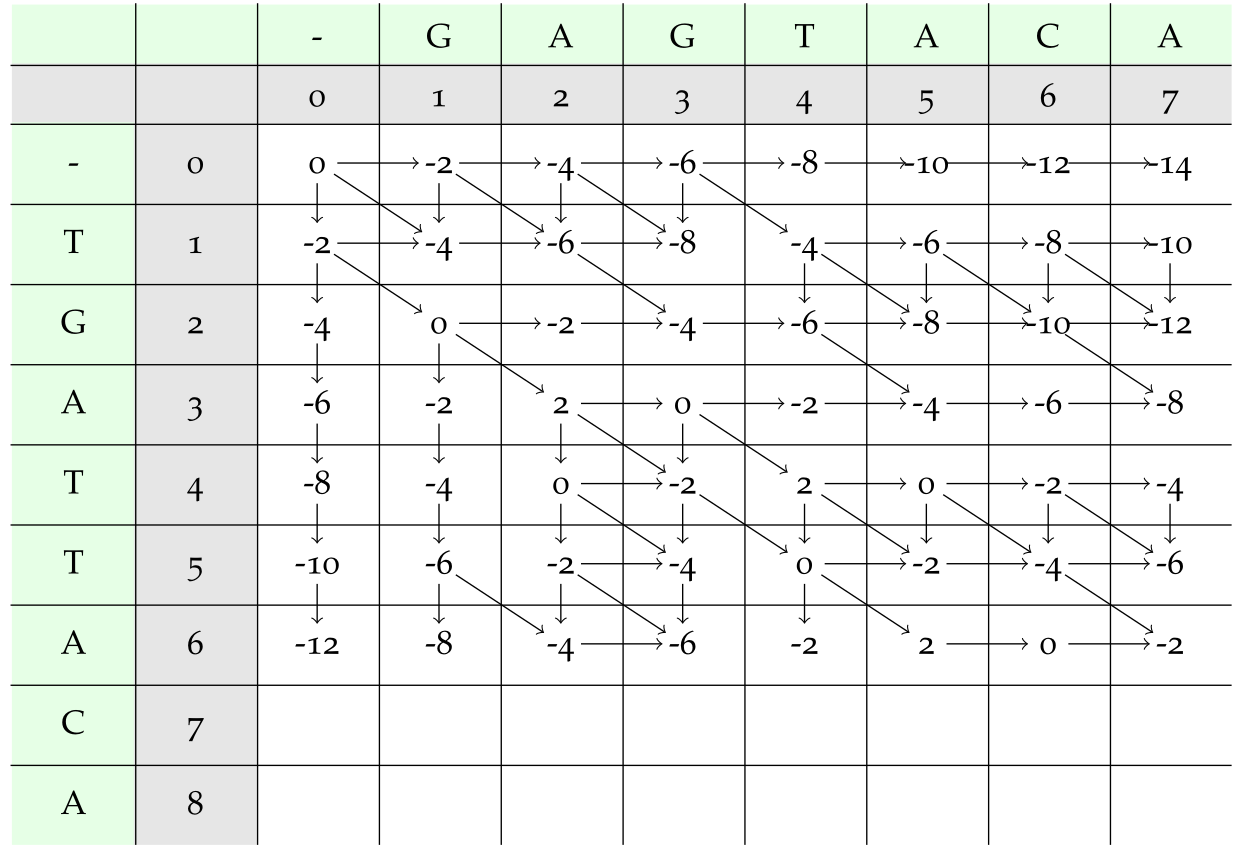
\includegraphics[scale=0.2]{NW-tabela.png}

				\textit{Dopolnite tabelo tako, da poračunate vrednosti (in ustrezne puščice) za zadnji dve vrstici.}

				\begin{center}
					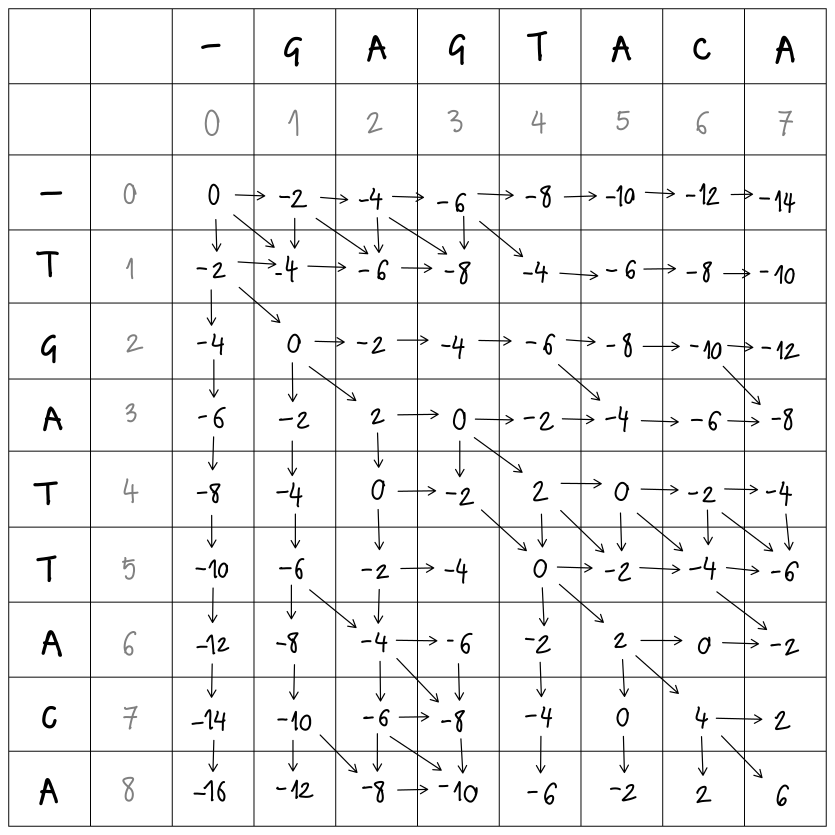
\includegraphics[scale=0.25]{matrika-complete-1.png}
				\end{center}

			\item \textit{Koliko optimalnih globalnih poravnav dobite? Izpišite vse rešitve.}

				Dobim dve optimalni globalni poravnavi, in sicer:

				\begin{multicols}{2}
					\begin{tabular}{c||c|c|c|c|c|c|c|c|c}
						s & - & G & A & G & T & - & A & C & A \\
						\hline
						t & T & G & A & - & T & T & A & C & A
					\end{tabular}

					\begin{tabular}{c||c|c|c|c|c|c|c|c|c}
						s & - & G & A & G & - & T & A & C & A \\
						\hline
						t & T & G & A & - & T & T & A & C & A
					\end{tabular}
				\end{multicols}

				Z matrikami to izgleda tako:

				\begin{multicols}{2}
					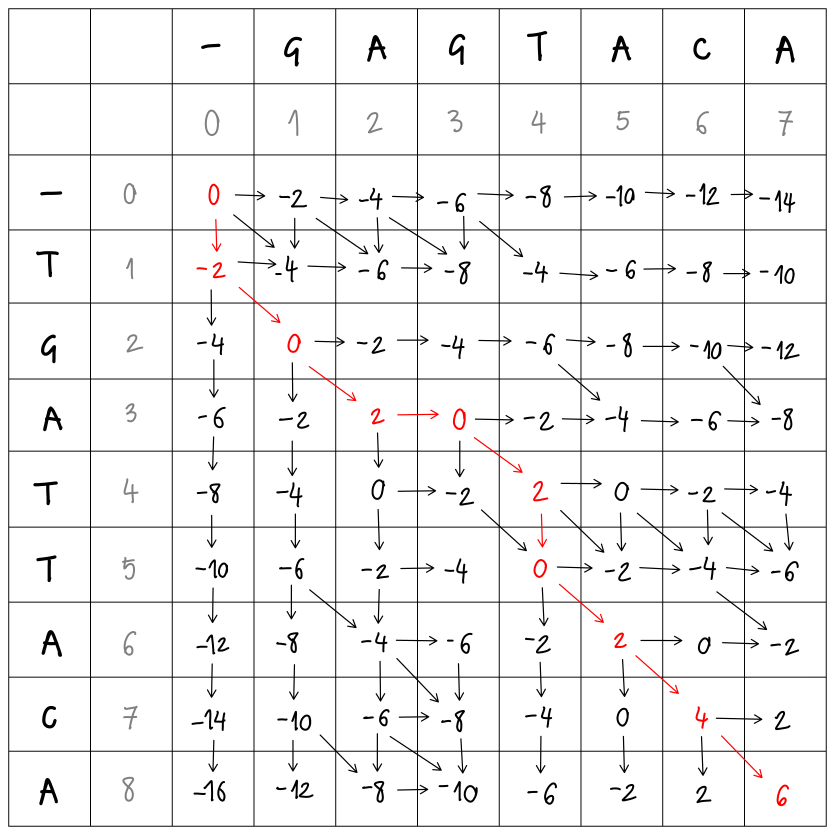
\includegraphics[scale=0.25]{matrika-complete-2}

					\columnbreak

					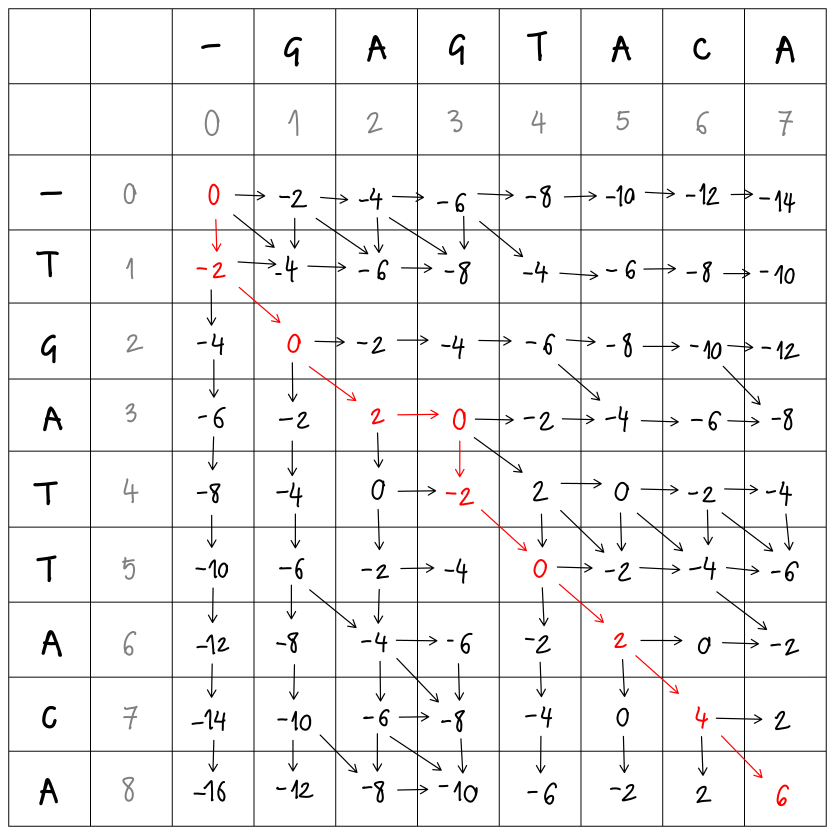
\includegraphics[scale=0.25]{matrika-complete-3}
				\end{multicols}

				Spremeni se mesto vrzeli in sicer iz mesta (4,4) na mesto (4,3).
		\end{enumerate}

	\item \textit{Dano imamo naslednjo matriko izražanja:}

		\begin{center}
			\begin{tabular}{c||c|c|c|c|c|c|}
				& $T_1$ & $T_2$ & $T_3$ & $T_4$ & $T_5$ & $T_6$ \\
				\hline
				\hline
				$g_1$ & 2 & 2 & 6 & 2 & 3 & 4 \\
				\hline
				$g_2$ & 3 & 7 & 3 & 1 & 9 & 3 \\
				\hline
				$g_3$ & 2 & 2 & 7 & 2 & 6 & 3 \\
				\hline
				$g_4$ & 3 & 2 & 3 & 2 & 1 & 3 \\
				\hline
				$g_5$ & 2 & 1 & 5 & 1 & 0 & 4 \\
				\hline
				$g_6$ & 3 & 5 & 5 & 8 & 2 & 3 \\
				\hline
				$g_7$ & 1 & 3 & 1 & 5 & 4 & 2 \\
				\hline
				$g_8$ & 5 & 4 & 2 & 4 & 7 & 5
			\end{tabular}
		\end{center}

	\item \textit{Določite gruče z uporabo metode voditeljev, če je začetna množica voditeljev
		enaka $X = \{g_1, g_5, g_6\}$.}

		Vsak gen lahko obravnavamo kot vektor $g_i = (T_1, \dots, T_6)$.

		\paragraph{Prva iteracija}
		\paragraph{Prvi korak} Najprej je potrebno izračunati razdalje med geni.
		(Evklidska) razdalja med vsakim genom je definirana kot:

		$$
		d(g_i, g_j) = \sqrt{ \left(T_{i}^{(1)} - T_{j}^{(1)} \right)^2 + \dots + \left(T_{i}^{(6)} - T_{j}^{(6)} \right)^2 } \quad ; \quad 1 \leq i,j \leq 8
		$$

		Primer za prvi gen:

		$$
		d(g_1, g_1) = \sqrt{ (2-2)^2 + (2-2)^2 + (6-6)^2 + (2-2)^2 + (3-3)^2 + (4-4)^2 } = 0
		$$

		Očitno je razdalja med istim genom 0, kar pravi tudi prva lastnost metrike: $d(x,y) = 0 \iff x = y$.

		Ko poračunamo vse, dobimo matriko razdalj. Potrebujemo razdalje samo do voditeljev:

		\begin{center}
			\begin{tabular}{c||c|c|c|}
				& $d(g_1, g_i)$ & $d(g_5, g_i)$ & $d(g_6, g_i)$ \\
				\hline
				\hline
				$g_1$ & 0 & 18.166 & 17.493\\
				\hline
				$g_2$ & 8.544 & 11.091 & 10.296\\
				\hline
				$g_3$ & 3.317 & 6.557 & 8.124\\
				\hline
				$g_4$ & 3.873 & 3.000 & 7.071\\
				\hline
				$g_5$ & 18.166 & 0 & 10.198\\
				\hline
				$g_6$ & 17.493 & 10.198 & 0\\
				\hline
				$g_7$ & 5.657 & 7.071 & 5.568\\
				\hline
				$g_8$ & 7.071 & 9.274 & 7.681\\
			\end{tabular}
		\end{center}

		\paragraph{Drugi korak} Za vsak gen izberemo najkrajšo razdaljo med njim in voditeljem.

		\begin{center}
			\begin{tabular}{c||c|c|c|}
				& $d(g_1, g_i)$ & $d(g_5, g_i)$ & $d(g_6, g_i)$ \\
				\hline
				\hline
				$g_1$ & \textcolor{red}{0} & 18.166 & 17.493\\
				\hline
				$g_2$ & \textcolor{red}{8.544} & 11.091 & 10.296\\
				\hline
				$g_3$ & \textcolor{red}{3.317} & 6.557 & 8.124\\
				\hline
				$g_4$ & 3.873 & \textcolor{red}{3.000} & 7.071\\
				\hline
				$g_5$ & 18.166 & \textcolor{red}{0} & 10.198\\
				\hline
				$g_6$ & 17.493 & 10.198 & \textcolor{red}{0}\\
				\hline
				$g_7$ & 5.657 & 7.071 & \textcolor{red}{5.568}\\
				\hline
				$g_8$ & \textcolor{red}{7.071} & 9.274 & 7.681\\
			\end{tabular}
		\end{center}

		\paragraph{Tretji korak} Iz vsakega stolpca odčitamo nove voditelje (vrednosti označene z
		rdečo), katere označimo s $C_i, i \in\mathbb{N}$, in sicer:

		\begin{align*}
			C_1 &= \left\{ g_1, g_2, g_3, g_8 \right\} \\
			C_2 &= \left\{ g_4, g_5 \right\} \\
			C_3 &= \left\{ g_6, g_7 \right\}
		\end{align*}

		\paragraph{Četrti korak} Za gručo $C_i$ z $n$ geni $\left\{ g_1, \dots, g_{k} \ | \ 1 \leq k \leq 8 \right\}$,
		izračunamo nov vektor vrednosti $v_i = \left( v_{i1}, \dots, v_{in} \right)$ z enačbo:

		$$
		v_{i} = \frac{ 1 }{ n} \sum_{j=1}^{n} g_{k}
		$$

		Nove vrednosti so torej aritmetična sredina vseh genov v gruči:

		\begin{align*}
			v_1 &= ( 3,   3.75, 4.5, 2.25, 6.25, 3.75 ) \\
			v_2 &= ( 2.5, 1.5,  4,   1.5,  0.5,  3.5 ) \\
			v_3 &= ( 2,   4,    3.5, 6.5,  3,    2.5 )
		\end{align*}

		Zdaj ponovimo korake dokler ne dosežemo \textbf{konvergence}:

		\begin{itemize}
			\item ko se gruče med iteracijama ne spremenijo
			\item ko postanejo razlike med radaljami gruč manjše od neke vnaprej določene vrednosti.
		\end{itemize}

		\paragraph{Druga iteracija}
		\paragraph{Prvi + drugi korak}

		\begin{center}
			\begin{tabular}{c||c|c|c|}
				& $d(v_1, g_i)$ & $d(v_2, g_i)$ & $d(v_3, g_i)$ \\
				\hline
				\hline
				$g_1$ & \textcolor{red}{3.808} & 3.354 & 5.723\\
				\hline
				$g_2$ & \textcolor{red}{4.743} & 10.209 & 8.761\\
				\hline
				$g_3$ & \textcolor{red}{3.317} & 6.344 & 6.764\\
				\hline
				$g_4$ & 5.788 & \textcolor{red}{1.500} & 5.454\\
				\hline
				$g_5$ & 7.036 & \textcolor{red}{1.500} & 7.263\\
				\hline
				$g_6$ & 7.314 & 7.632 & \textcolor{red}{2.784}\\
				\hline
				$g_7$ & 5.148 & 5.958 & \textcolor{red}{2.784}\\
				\hline
				$g_8$ & \textcolor{red}{3.937} & 8.185 & 6.305\\
			\end{tabular}
		\end{center}

		\paragraph{Tretji korak}

		\begin{align*}
			C_4 &= \left\{ g_1, g_2, g_3, g_8 \right\} \\
			C_5 &= \left\{ g_4, g_5 \right\} \\
			C_6 &= \left\{ g_6, g_7 \right\}
		\end{align*}

		Ker so gruče enake kot v prejšnji iteraciji, lahko postopek tu končamo\dots

		\textbf{Rešitev:} gruče določene z metodo voditeljev s $k=3$ za dano matriko
		izražanja so

		\begin{align*}
				&\left\{ g_1, g_2, g_3, g_8 \right\}  \\
				&\left\{ g_4, g_5 \right\}  \\
				&\left\{ g_6, g_7 \right\}
		\end{align*}

	\item \textit{Izračunajte drevo hierarhičnega gručenja z uporabo algoritma UPGMA.}

		Osnova za algoritem UPGMA je matrika razdalj genov (matrika iz prve iteracije
		prejšnje naloge), za katero uporabimo sledečo enačbo

		$$
		d_{\text{avg}}(C, C^*) = \frac{ 1 }{ |C| |C^*| } \sum_{x\in C, y\in C^*} d(x,y)
		$$

		kjer sta $C$ in $C^*$ dve gruči (na začetku so to geni).

		\begin{center}
			\begin{tabular}{c||c|c|c|c|c|c|c|c|}
				& $g_1$ & $g_2$ & $g_3$ & $g_4$ & $g_5$ & $g_6$ & $g_7$ & $g_8$ \\
				\hline
				\hline
				$g_1$ & 0     & 8.544 & 3.317 & 3.873 & 3.464 & 7.000 & 5.657 & 7.071 \\
				\hline
				$g_2$ &       & 0     & 8.124 & 10.198 & 11.091 & 10.296 & 10.677 & 8.602 \\
				\hline
				$g_3$ &       &       & 0     & 6.325 & 6.557  & 8.124  & 6.403 & 7.000 \\
				\hline
				$g_4$ &       &       &       & 0     & 3.000  & 7.071  & 5.099 & 6.403 \\
				\hline
				$g_5$ &       &       &       &       & 0      & 10.198 & 7.071 & 9.274 \\
				\hline
				$g_6$ &       &       &       &       &        & 0      & 5.568 & 7.681 \\
				\hline
				$g_7$ &       &       &       &       &        &        & 0     & 5.916 \\
				\hline
				$g_8$ &       &       &       &       &        &        &        & 0     \\
			\end{tabular}
		\end{center}

		Gručenje deluje tako, da vsako iteracijo izberemo najbližja gena in ju združimo
		v gručo. Na začetku je vsak gen v svoji gruči, do konca postopka pa ustvarimo eno
		celovito gručo, ki bo vsebovala vse gene.

		Začetni dendrogram:

		\begin{tikzpicture}[sloped]
			\node (1) at (-7,0) {$g_1$};
			\node (2) at (-5,0) {$g_2$};
			\node (3) at (-3,0) {$g_3$};
			\node (4) at (-1,0) {$g_4$};
			\node (5) at (1,0) {$g_5$};
			\node (6) at (3,0) {$g_6$};
			\node (7) at (5,0) {$g_7$};
			\node (8) at (7,0) {$g_8$};
		\end{tikzpicture}

		\paragraph{Prvi korak} Izberemo najmanjšo vrednost med razdaljami.

		\begin{center}
			\begin{tabular}{c||c|c|c|c|c|c|c|c|}
				& $g_1$ & $g_2$ & $g_3$ & $g_4$ & $g_5$ & $g_6$ & $g_7$ & $g_8$ \\
				\hline
				\hline
				$g_1$ & 0     & 8.544 & 3.317 & 3.873 & 3.464 & 7.000 & 5.657 & 7.071 \\
				\hline
				$g_2$ &       & 0     & 8.124 & 10.198 & 11.091 & 10.296 & 10.677 & 8.602 \\
				\hline
				$g_3$ &       &       & 0     & 6.325 & 6.557  & 8.124  & 6.403 & 7.000 \\
				\hline
				$g_4$ &       &       &       & 0     & \textcolor{red}{3.000}  & 7.071  & 5.099 & 6.403 \\
				\hline
				$g_5$ &       &       &       &       & 0      & 10.198 & 7.071 & 9.274 \\
				\hline
				$g_6$ &       &       &       &       &        & 0      & 5.568 & 7.681 \\
				\hline
				$g_7$ &       &       &       &       &        &        & 0     & 5.916 \\
				\hline
				$g_8$ &       &       &       &       &        &        &        & 0     \\
			\end{tabular}
		\end{center}

		\paragraph{Drugi korak} Dodamo gena v gručo $C_1$, torej $C_1 = \{g_4, g_5\}$ in poračunamo
		novi vektor $v_1$, ki bo predstavljal novo gručo v matriki razdalj (tako kot prej uporabimo
		aritmetično sredino komponent):

		$$
		v_1 = (2.5, 1.5, 4, 1.5, 0.5, 3.5)
		$$

		\paragraph{Tretji korak} Izračunamo razdaljo gruče ($C$) do vseh ostalih gruč
		($C^*$) s pomočjo prejšnje enačbe. V matriki razdalj odstranimo gena, ki smo ju združili
		v gručo ter dodamo novo gručo:

		\begin{center}
			\begin{tabular}{c||c|c|c|c|c|c|c|}
				& $g_1$ & $g_2$ & $g_3$ & $C_1$ & $g_6$ & $g_7$ & $g_8$ \\
				\hline
				\hline
				$g_1$ & 0     & 8.544 & 3.317 & 3.669 & 7.000 & 5.657 & 7.071 \\
				\hline
				$g_2$ &       & 0     & 8.124 & 10.645& 10.296 & 10.677 & 8.602 \\
				\hline
				$g_3$ &       &       & 0     & 6.441 & 8.124  & 6.403 & 7.000 \\
				\hline
				$C_1$ &       &       &       & 0     & 8.635  & 6.085 & 7.839 \\
				\hline
				$g_6$ &       &       &       &       & 0      & 5.568 & 7.681 \\
				\hline
				$g_7$ &       &       &       &       &        & 0     & 5.916 \\
				\hline
				$g_8$ &       &       &       &       &        &        & 0     \\
			\end{tabular}
		\end{center}

		\paragraph{Četrti korak} Gena povežemo na dendrogramu na izračunani višini:

		\begin{tikzpicture}[sloped]
			\node (1) at (-7,0) {$g_1$};
			\node (2) at (-5,0) {$g_2$};
			\node (3) at (-3,0) {$g_3$};
			\node (4) at (-1,0) {$g_4$};
			\node (45) at (-1,0) {$g_4$};
			\node (5) at (1,0) {$g_5$};
			\node (6) at (3,0) {$g_6$};
			\node (7) at (5,0) {$g_7$};
			\node (8) at (7,0) {$g_8$};

			\draw (4) |- (5.center);
		\end{tikzpicture}

\end{enumerate}
\end{document}
